% vim:ft=tex
% rubber: module xelatex

\subsection{Face recognition}
\label{sec:face-rec}
We have implemented face recognition based on PCA analysis of the image pixel
values (the holistic approach). Face recognition is effectively the culmination of all our work so far.

Our first step is to preprocess the image database. Images must first be rectified (see section~\ref{sec:rectification}). Preprocessing ensures that a fixed triple of face features (the outer corners of the eyes, and the point between the base of the nose and the lip) are in the same positions for all images. For further details, see section~\ref{sec:preprocess} below. PCA is performed on these processed images.

Up to six channels of data from each image can be used: values for red, green and blue, values for hue and saturation, and depth values. Depth values are created by running our stereo matching algorithm (see section~\ref{sec:stereo}) on the preprocessed images to create equivalent-sized depth maps.\footnote{ It is important at this step to use a fixed multiplier for disparities in all the images, rather than dynamically calculating how to best map the disparities in an image to [0...255]. This is so that representations of relative distances are fixed across all images in the dataset.}

For each pixel in the image in turn, the $n$ data points are concatenated into a series of values, and appended to the single column image vector. The result is a single vector of length $L = n \times m$, where $m$ is the total number of pixels in the image.

For the training phase of the PCA processing, the average image vector for the
training set is computed, and subtracted from each image vector to create the normalised vectors. Each vector is multiplied by its inverse, and the resulting matrices are summed to acquire the overall covariance matrix. This matrix essentially holds all the information of the database of images.

The next step requires that the eigenvectors and eigenvalues of the matrix be calculated. Because the size of the matrix is $L^{2}$, this is computationally expensive. We were able to achieve reduction of dimensionality by using the OpenCV PCA library functions in our code. OpenCV implements the variation introduced by \citet{turk_pentland}, whereby the eigenvectors and eigenvalues are calculated by a square matrix whose dimensionality is equal to the the number of images in the database - a considerable reduction. This allows us to achieve training and matching in a reasonable time and with reasonable memory consumption.

The highest eigenvalues represent those components (`directions') for which we have the greatest variance, i.e. discriminating power. The eigenvectors associated with those highest eigenvalues are kept. The number to keep is a user-configurable parameter. The program calculates the fractional quantity $Q$ of face information being stored by dividing the sum of the \emph{kept} eigenvalues by the sum of \emph{all} the eigenvalues. The user can therefore trade off efficiency (in terms of memory and time) against quality by choosing to keep a number of components such that $Q \geq t$ for some threshold $t$.

The result is a set of eigenvectors which give us an orthonormal basis, or higher-dimensional `principal component space'. Each training image is projected into this space, and for each class of images (i.e. each person whose image was taken), the \emph{average image vector} (in the principal component space) is computed. The maximum distance between
the average image and the set of original training images for that class is also calculated. This maximum distance
(multiplied by some user-configurable factor) is used as a cutoff distance when
matching; images that do not match any classes within the cutoff distance are
considered a no-match.

The program uses this same metric to gauge the confidence in a prediction. Images which, when projected into the orthonormal basis, are close to the edge of the `point cloud' of training examples for the closest-fitting class, are less likely to have been \emph{correctly} matched to that class than those very near to the average image vector.

To test the accuracy of the classification, each training image is projected
into the eigenspace and back; the error between the original image and the
reconstructed image (as the square of the distance) is calculated. Sample results for
this are shown in section~\ref{sec:pcaresults} below.

When given an image to classify, matching is performed as follows. The image vector is constructed as for the training set, using $n$ channels and resulting in a vector length $n \times image-height \times image-width$. The overall average vector is subtracted from the image vector, which is then projected into the PCA space. The distance of this projection to each class average vector is computed. The class vector that is nearest to the test image is considered a match if it is closer than the cutoff depth for that class. Our program by default returns the closest match and the next-closest match, stating the confidence in each guess.

\subsubsection{Preprocessing of images}
\label{sec:preprocess}

Before doing PCA analysis on the face images, they are preprocessed or `registered' to make sure
face features are in (almost) the same positions on all the images. Initially, we operate on rectified images, i.e. stereo images that have
been projected into a geometry in which they have corresponding horizontal epipolar lines. The
rectification step helps diminish unwanted deformation caused by the later steps of the
preprocessing, and also prepares the images for stereo mapping if we wish to use depth data for PCA.

After rectification, face features are manually identified. The features
identified are the outer corners of the eyes, and the point above the lip on the vertical centre of the nose
(since these features are fairly definable, and seem to be in approximately the same position regardless
of facial expression). For each of these feature points $p$, the average $p'$of each feature point over the whole image
training database is found. Each image is geometrically transformed so that its three feature points align to the location of $p'$.

This is done by solving (for each image) the affine transformation needed to transform the feature point
locations for that image into the average location $p'$, using singular value
decomposition of the resulting set of matrices. This is applied as an affine
transformation to the whole image. Pixel interpolation is performed to create the new image. All three steps are done using OpenCV functions.

Following the transformation, the images are cropped to a user-configurable
ratio. The ratio is determined by adding some factor of the vertical and horizontal distances
between the feature points to the edges of the image. An ellipse is then fitted to the boundaries of the cropped image. Everything outside this ellipse is
`blacked out' to zero values. Finally, the image is scaled down to a fixed width (also
user-configurable), to speed up the processing.

Finally, we apply our stereo matching implementation to the processed images to
yield the depth map that can optionally be used in the PCA matching. The last channels - Hue and Saturation values - are extracted from each pixel by a function during the processing.

\subsubsection{Testing face recognition}
\label{sec:pcaresults}

We tested our face recognition processor in various ways. Our methodology involved, for each test, using whichever number of principal components meant keeping at least 80\% image information (in terms of fraction of the total eigenvalues). We set the error threshold to a relatively strict $1.0$, i.e. the system would only identify a test image as belonging to some class $C$ if the variation between the image and the mean of $C$ was less than or equal to the maximum variation within the training images for that class. For each experiment, we used half our face database of 88 images to train, and half to test. There are 11 classes in the database, and approximately the same number of images per class.

We first look at the amount of image data being retained by PCA. Consider table~\ref{tbl:face-rec-1}. The amount of information being retained when a certain number of components are kept is not very dependent on the image size: there is little difference between the various tested sizes, even when we use images $\frac{1}{64}$ the size of our main dataset. In all cases, 12 or 13 components are required to achieve the 80\% information retention threshold which we use in our other experiments.

\begin{table}[htbp]
  \centering
  \begin{tabular}{c c c c c}
    \toprule
    & \multicolumn{4}{c}{\textbf{Image size}} \\
      &  32x49  &  64x99  & 128x198 & 256x396 \\
    \midrule
    \textbf{2 components} & 39.6\% & 39.9\% & 38.8\% & 37.8\% \\
    \textbf{4 components} & 55.6\% & 56.0\% & 55.5\% & 53.2\% \\
    \textbf{6 components} & 64.8\% & 65.2\% & 64.0\% & 62.2\% \\
    \textbf{8 components} & 71.9\% & 72.4\% & 70.5\% & 69.3\% \\
    \textbf{10 components} & 77.2\% & 77.6\% & 76.1\% & 74.6\% \\
    \textbf{12 components} & 80.8\% & 81.3\% & 79.8\% & 78.4\% \\
    \textbf{14 components} & 83.8\% & 84.4\% & 82.3\% & 81.6\% \\
    \textbf{16 components} & 86.3\% & 86.8\% & 85.7\% & 84.2\% \\
    \bottomrule
  \end{tabular}
  \caption[Information retained in face recognition tests for different-sized images]{Information retained in face recognition tests for different-sized images. Each row is a case where a different number of components were kept. Each column is a different image dimensionality. Results are presented as percentage of total summed eigenvalues. In each case, PCA was performed on all six possible channels, on a training set of 44 images with 11 classes.}
  \label{tbl:face-rec-1}
\end{table}

We are able to reconstruct images by projecting them into and then out of the PCA basis. Table~\ref{tbl:face-rec-2} shows the effects of this reconstruction for our training images. As we would obviously expect, we have better reconstruction when we keep more principal components. The total improvement when we increase from 4 components to 10 is $41695$. The total improvement when we go from 10 components to 16 is $12489$. This apparent case of diminishing returns is due to the way PCA works: we begin by including more `important' (in terms of their associated eigenvalue) eigenvectors, and then start adding ones which lend less to the PCA process. Therefore the more principal components we add, the less additional improvement we see.

\begin{table}[htpb]
  \centering
  \begin{tabular}{c c c c}
    \toprule
     & \textbf{4 components} & \textbf{10 components} & \textbf{16 components} \\
     & (53.2\% data retained) & (74.6\% data retained) & (84.2\% data retained) \\
    \midrule
    \textbf{Class A} & 9848 & 9018 & 6670\\
    \textbf{Class B} & 11238 & 7853 & 6170\\
    \textbf{Class C} & 11719 & 7811 & 7376\\
    \textbf{Class D} & 12061 & 7736 & 6560\\
    \textbf{Class E} & 10268 & 7873 & 6383\\
    \textbf{Class F} & 13339 & 8683 & 7001\\
    \textbf{Class G} & 10252 & 9022 & 6516\\
    \textbf{Class H} & 14167 & 7331 & 5709\\
    \textbf{Class I} & 11945 & 10223 & 7379\\
    \textbf{Class J} & 11196 & 9187 & 6075\\
    \textbf{Class K} & 11586 & 8267 & 7596\\
    \bottomrule
  \end{tabular}
  \caption[Sample reconstruction error for the 256x396 size images]{Sample reconstruction error for the 256x396 size images, with PCA performed on all six possible channels. A training set of 44 images with 11 classes was used. Each column is the error for one class (person) in the training set. Error is measured in absolute difference between the original training example image vector and the reconstructed vector projected back out of the PCA space. Each row is a case where a different number of components were kept, with the quantity of information retained (as a percentage of total summed eigenvalues) in brackets.}
  \label{tbl:face-rec-2}
\end{table}

Examples of reconstructed images are given in figure~\ref{fig:reconstructed-means}. The first two cases are the authors' reconstructed class mean eigenfaces, and the second two are the overall reconstructed mean eigenface, and the overall reconstructed mean eigenface for a different database.

\begin{figure}[htb]
 \centering
 \subfloat[Class mean \#1] { \label{fig:classm-1} 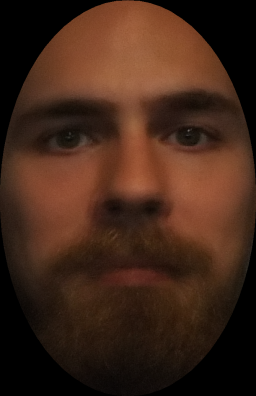
\includegraphics[trim = -2mm -2mm -2mm -2mm, width=0.2\textwidth]{example/PCA_class_mean_b} }
 \subfloat[Class mean \#2] { \label{fig:classm-2} 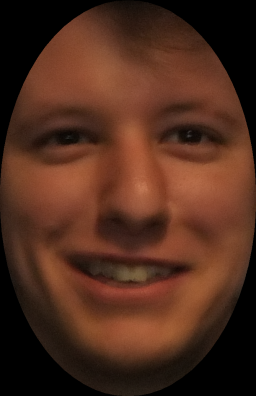
\includegraphics[trim = -2mm -2mm -2mm -2mm, width=0.2\textwidth]{example/PCA_class_mean_c} }
 \subfloat[Database mean] { \label{fig:classm-3} 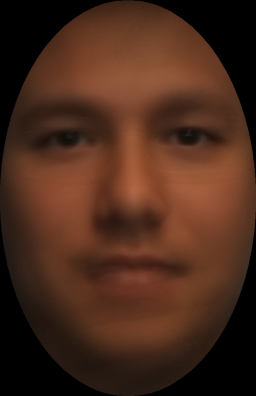
\includegraphics[trim = -2mm -2mm -2mm -2mm, width=0.2\textwidth]{example/OVERALL_PCA_MEAN} }
 \subfloat[Other database mean] { \label{fig:classm-4} 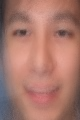
\includegraphics[trim = -2mm -2mm -2mm -2mm, width=0.2\textwidth]{example/OVERALL_PCA_MEAN_PREV} }\\
 \caption[Examples of reconstructed images]{Examples of reconstructed images for class means and overall database means. The mean eigenface for a previous year's database is given at the far right for comparison. PCA was performed with 12 principal components retained to create these images, each of which is the reconstruction of the mean of four training examples.}
 \label{fig:reconstructed-means}
\end{figure}

Table~\ref{tbl:face-rec-3} presents our accuracy results of the system for databases of different image sizes. We observed that most often, PCA failed on the classes or test images for the person whose hand was over his face, the person who had the most different positions and expressions, the person who had only two training images, and the person wearing a hat. These are classes F, C, H, K respectively in Table~\ref{tbl:face-rec-2}. Very few test images outside of these unexpected cases were misclassified or unclassified. Note that classes F and H have the highest reconstruction error when only a few components are kept: PCA is unable to reconstruct the considerable variance \emph{within} the class at a lower dimensionality.

In general, though, we observe that those classes of images with the greatest variance in pose, lighting or expression are \emph{not necessarily} the hardest to classify. It simply means that we have less confidence when we classify into that class. These highly varying images did, however, result in a broad `point cloud' in higher-dimensional PCA space, so when any test image was misclassified, it had a greater-than-average chance to be misclassified into a highly varying class.

\begin{table}[bp]
  \centering
  \begin{tabular}{>{\centering}m{2cm} >{\centering}m{1.5cm} >{\centering}m{1.5cm}
      >{\centering}m{1.5cm} >{\centering}m{1.5cm} }
    \toprule
     & \multicolumn{4}{c}{\textbf{Image size}} \tabularnewline
    &  32x49  &  64x99  & 128x198 & 256x396 \tabularnewline
    \midrule
    \textbf{Successfully classified} & 30 & 32 & 33 & 34 \tabularnewline
    \cmidrule{1-1}
    \textbf{Failed to classify} & 14 & 9 & 7 & 4 \tabularnewline
    \cmidrule{1-1}
    \textbf{Partially misclassified} & 0 & 2 & 3 & 4 \tabularnewline
    \cmidrule{1-1}
    \textbf{Completely misclassified} & 0 & 1 & 1 & 2 \tabularnewline
    \bottomrule
  \end{tabular}
  \caption[Results of classification testing for different-sized images]{Results of using PCA for face recognition of new images (classification testing). Four different image sizes are tested. A training set of 44 images with 11 classes was used, and in all cases, PCA was performed on all six possible channels. A number of principal components sufficient to retain 80\% image data were used. Each column is a different image dimensionality. `Number successfully classified' is the number of test images correctly classified. `Number failed to classify' is the number of test images the processor was not confident enough to enter a guess for. `Number partially misclassified' is the number of test images for which the processor's second guess was correct. `Number completely misclassified' is the number of test images for which the processor's initial and secondary guesses were both incorrect.}
  \label{tbl:face-rec-3}
\end{table}

Note that, in Table~\ref{tbl:face-rec-3}, as we increase image size we see better classification. Furthermore, there is a slight trend away from complete \emph{failures to classify} and towards \emph{misclassifications}. At the biggest image size tested, more images are misclassified than are found unable to be classified.

\begin{table}[bp]
  \centering
  \begin{tabular}{>{\centering}m{2cm} >{\centering}m{1.5cm} >{\centering}m{1.5cm}
      >{\centering}m{1.5cm} >{\centering}m{1.5cm} }
    \toprule
    \textbf{ } & \textbf{ RGB } & \textbf{ RGB + HS } & \textbf{RGB + Depth} &
    \textbf{RGB + HS + Depth} \tabularnewline
    \midrule
    \textbf{Successfully classified} & 29 & 34 & 31 & 34 \tabularnewline
    \cmidrule{1-1}
    \textbf{Failed to classify} & 7 & 5 & 6 & 4 \tabularnewline
    \cmidrule{1-1}
    \textbf{Partially misclassified} & 5 & 4 & 5 & 4 \tabularnewline
    \cmidrule{1-1}
    \textbf{Completely misclassified} & 3 & 1 & 2 & 2 \tabularnewline
    \bottomrule
  \end{tabular}
  \caption[Results of classification testing for different numbers of channels]{Results of using PCA for face recognition of new images (classification testing), using different channels. RGB, HSV and depth map data are tested. Each column specifies a different combination. A training set of 44 images, of dimension 256x396, with 11 classes was used. `Number successfully classified' is the number of test images correctly classified. `Number failed to classify' is the number of test images the processor was not confident enough to enter a guess for. `Number partially misclassified' is the number of test images for which the processor's second guess was correct. `Number completely misclassified' is the number of test images for which the processor's initial and secondary guesses were both incorrect.}
  \label{tbl:face-rec-4}
\end{table}

Table~\ref{tbl:face-rec-4} shows the results of using different channels for PCA. In general, the more tracked data, the better. PCA generally worked well even with simple RGB data. While we cannot say so with statistical rigour, it does appear that the Hue and Saturation values may be more useful than the depth data. This may be because those disparity maps were created by stereo matching on \emph{preprocessed} images: the images began as rectified stereo pairs, but underwent an affine transformation before stereo matching. This means the depth map quality was noticeably lower than usual.

The beauty of the PCA process is that even if we were using random noise for depth maps, it would not matter: PCA will simply learn that those data values are not good discriminators (and therefore predictors); any eigenvector along the `direction(s)' of depth would not have a high eigenvalue, and therefore would not be chosen as a principal component.

These observations are only valid given our particular (relatively strict) cut-off point or `confidence tolerance' for classification. Some data channels might have proven themselves better or worse if we had required the system to return a guess for the class of every single test image, including those that are hard to classify.

\begin{figure}[hb]
 \centering

 \subfloat { \label{fig:row1-1} 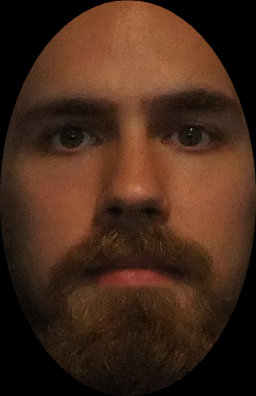
\includegraphics[trim = -1mm -1mm -1mm -1mm, width=0.12\textwidth]{classDB/A-norm} }
 \subfloat { \label{fig:row1-2} 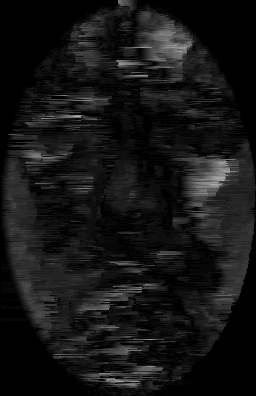
\includegraphics[trim = -1mm -1mm -1mm -1mm, width=0.12\textwidth]{classDB/A-norm-D} }
 \subfloat { \label{fig:row1-3} 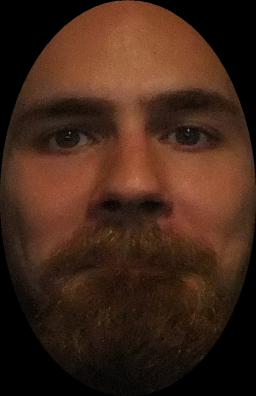
\includegraphics[trim = -1mm -1mm -1mm -1mm, width=0.12\textwidth]{classDB/B-norm} }
 \subfloat { \label{fig:row1-4} 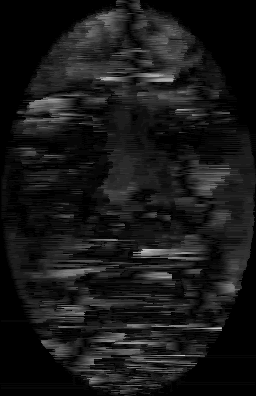
\includegraphics[trim = -1mm -1mm -1mm -1mm, width=0.12\textwidth]{classDB/B-norm-D} }\\

 \subfloat { \label{fig:row2-1} 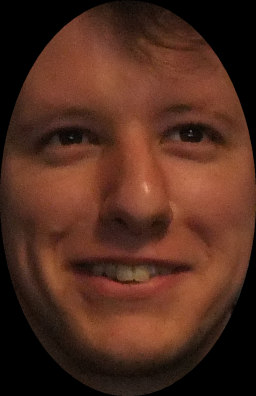
\includegraphics[trim = -1mm -1mm -1mm -1mm, width=0.12\textwidth]{classDB/C-norm} }
 \subfloat { \label{fig:row2-2} 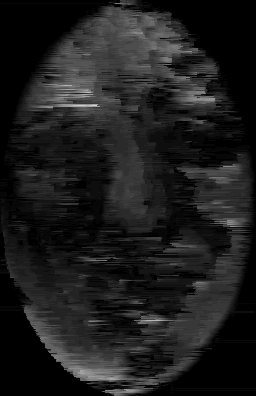
\includegraphics[trim = -1mm -1mm -1mm -1mm, width=0.12\textwidth]{classDB/C-norm-D} }
 \subfloat { \label{fig:row2-3} 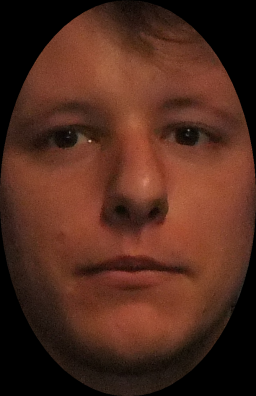
\includegraphics[trim = -1mm -1mm -1mm -1mm, width=0.12\textwidth]{classDB/D-norm} }
 \subfloat { \label{fig:row2-4} 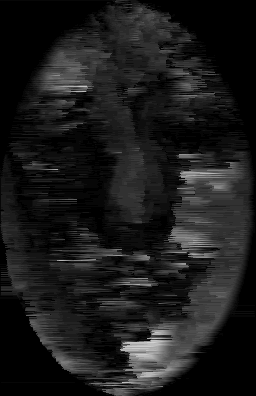
\includegraphics[trim = -1mm -1mm -1mm -1mm, width=0.12\textwidth]{classDB/D-norm-D} }\\

 \subfloat { \label{fig:row3-1} 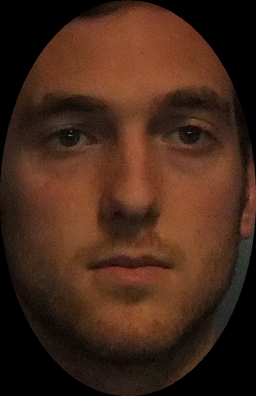
\includegraphics[trim = -1mm -1mm -1mm -1mm, width=0.12\textwidth]{classDB/E-norm} }
 \subfloat { \label{fig:row3-2} 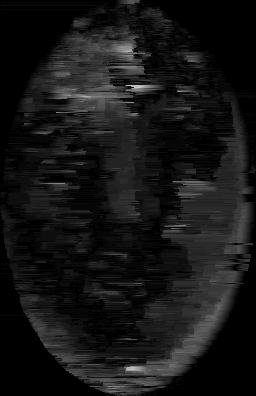
\includegraphics[trim = -1mm -1mm -1mm -1mm, width=0.12\textwidth]{classDB/E-norm-D} }
 \subfloat { \label{fig:row3-3} 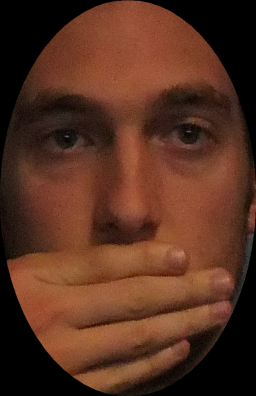
\includegraphics[trim = -1mm -1mm -1mm -1mm, width=0.12\textwidth]{classDB/F-norm} }
 \subfloat { \label{fig:row3-4} 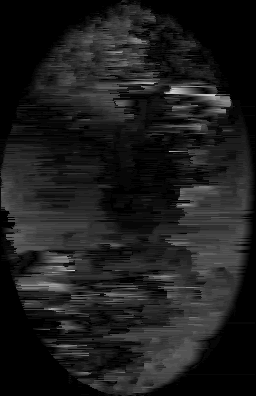
\includegraphics[trim = -1mm -1mm -1mm -1mm, width=0.12\textwidth]{classDB/F-norm-D} }\\

 \subfloat { \label{fig:row4-1} 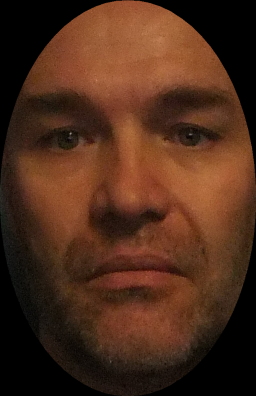
\includegraphics[trim = -1mm -1mm -1mm -1mm, width=0.12\textwidth]{classDB/G-norm} }
 \subfloat { \label{fig:row4-2} 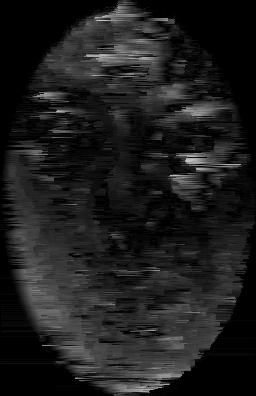
\includegraphics[trim = -1mm -1mm -1mm -1mm, width=0.12\textwidth]{classDB/G-norm-D} }
 \subfloat { \label{fig:row4-3} 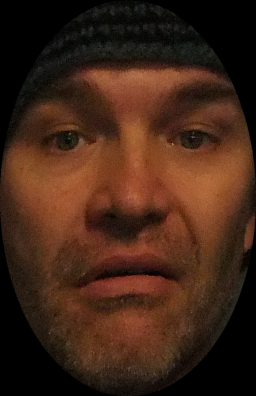
\includegraphics[trim = -1mm -1mm -1mm -1mm, width=0.12\textwidth]{classDB/H-norm} }
 \subfloat { \label{fig:row4-4} 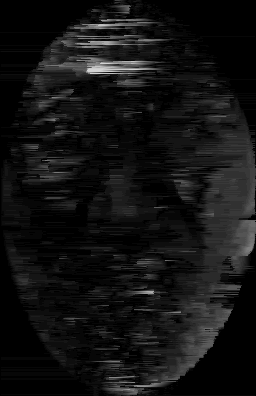
\includegraphics[trim = -1mm -1mm -1mm -1mm, width=0.12\textwidth]{classDB/H-norm-D} }\\

 \caption[A sample of our PCA database]{A sample of images from our PCA database. Each row of images
describes two images from a class, alongside their associated depth map. These are the rectified,
registered $256\times396$ resolution images taken with the W3 camera.}
 \label{fig:classdb}
\end{figure}
